\begin{frame}[allowframebreaks]{Predict missing pieces}
    \begin{figure}
        \flushleft
        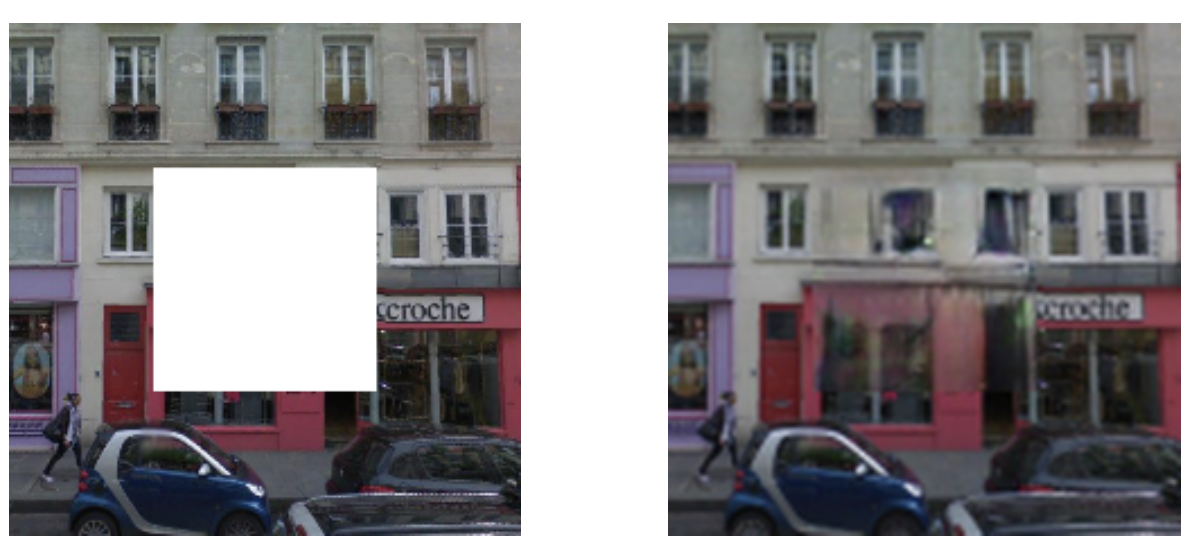
\includegraphics[width=1\linewidth,height=\textheight,keepaspectratio]{images/ssl/slide_17_1_img.png}
        \footnote{Pathak et al. (2016), "Context Encoders: Feature Learning by Inpainting," CVPR 2016.}
    \end{figure}
\end{frame}


\begin{frame}[allowframebreaks]{Context Encoders}
    \textbf{Context Encoders} are designed to learn meaningful image representations by reconstructing missing parts of an image.

    \vspace{0.15em}
    \textbf{Key Idea:}
    \begin{itemize}
        \setlength{\itemsep}{-0.5em}
        \item Randomly mask or remove patches from an input image.
        \item Use an encoder–decoder neural network to predict and reconstruct the missing content.
        \item The model is trained to minimize the difference between the predicted and actual image patches.
    \end{itemize}

    \vspace{0.15em}
    \textbf{Architecture:}
    \begin{itemize}
        \setlength{\itemsep}{-0.5em}
        \item \textbf{Encoder:} Processes the visible parts of the image and extracts feature representations.
        \item \textbf{Decoder:} Generates the missing image regions based on the encoded features.
        \item The entire network is trained end-to-end using a reconstruction loss (e.g., L2 loss).
    \end{itemize}

    \framebreak

    \begin{figure}
        \flushleft
        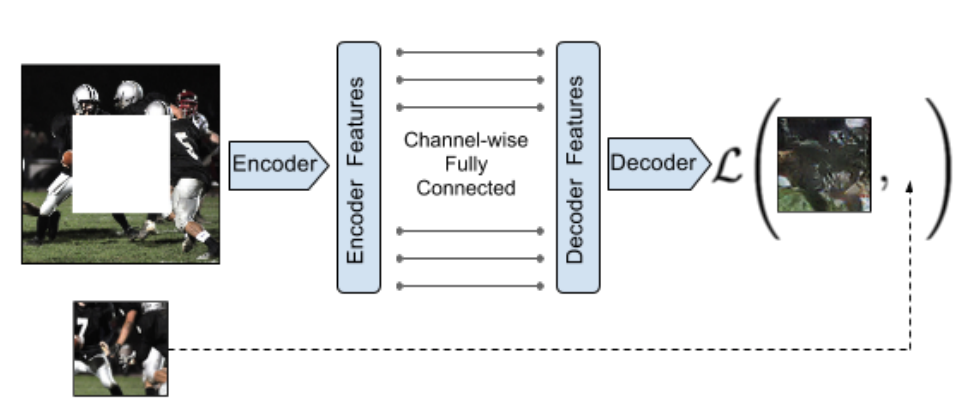
\includegraphics[width=1\linewidth,height=\textheight,keepaspectratio]{images/ssl/slide_18_1_img.png}
    \end{figure}

    \framebreak

    \begin{figure}
        \flushleft
        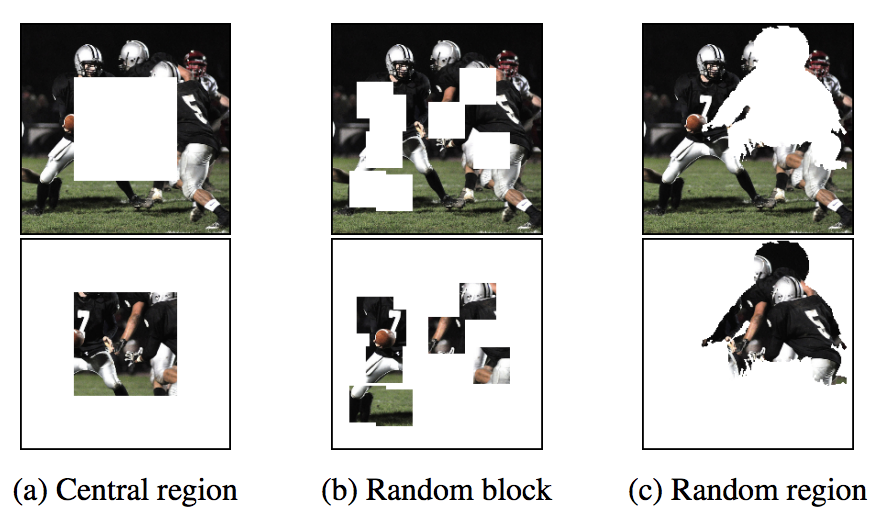
\includegraphics[width=1\linewidth,height=\textheight,keepaspectratio]{images/ssl/slide_19_1_img.png}
    \end{figure}

    \framebreak

    \begin{figure}
        \flushleft
        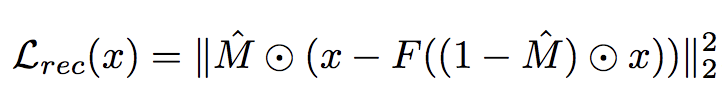
\includegraphics[width=1\linewidth,height=\textheight,keepaspectratio]{images/ssl/slide_20_3_img.png}
    \end{figure}

    \begin{figure}
        \flushleft
        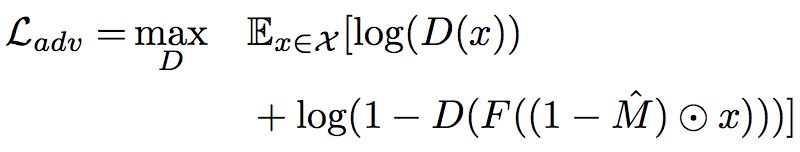
\includegraphics[width=1\linewidth,height=\textheight,keepaspectratio]{images/ssl/slide_20_2_img.png}
    \end{figure}

    \begin{figure}
        \centering
        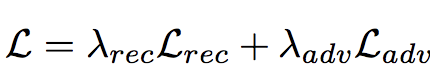
\includegraphics[width=0.7\linewidth,height=\textheight,keepaspectratio]{images/ssl/slide_20_1_img.png}
    \end{figure}

    \framebreak

    \begin{figure}
        \flushleft
        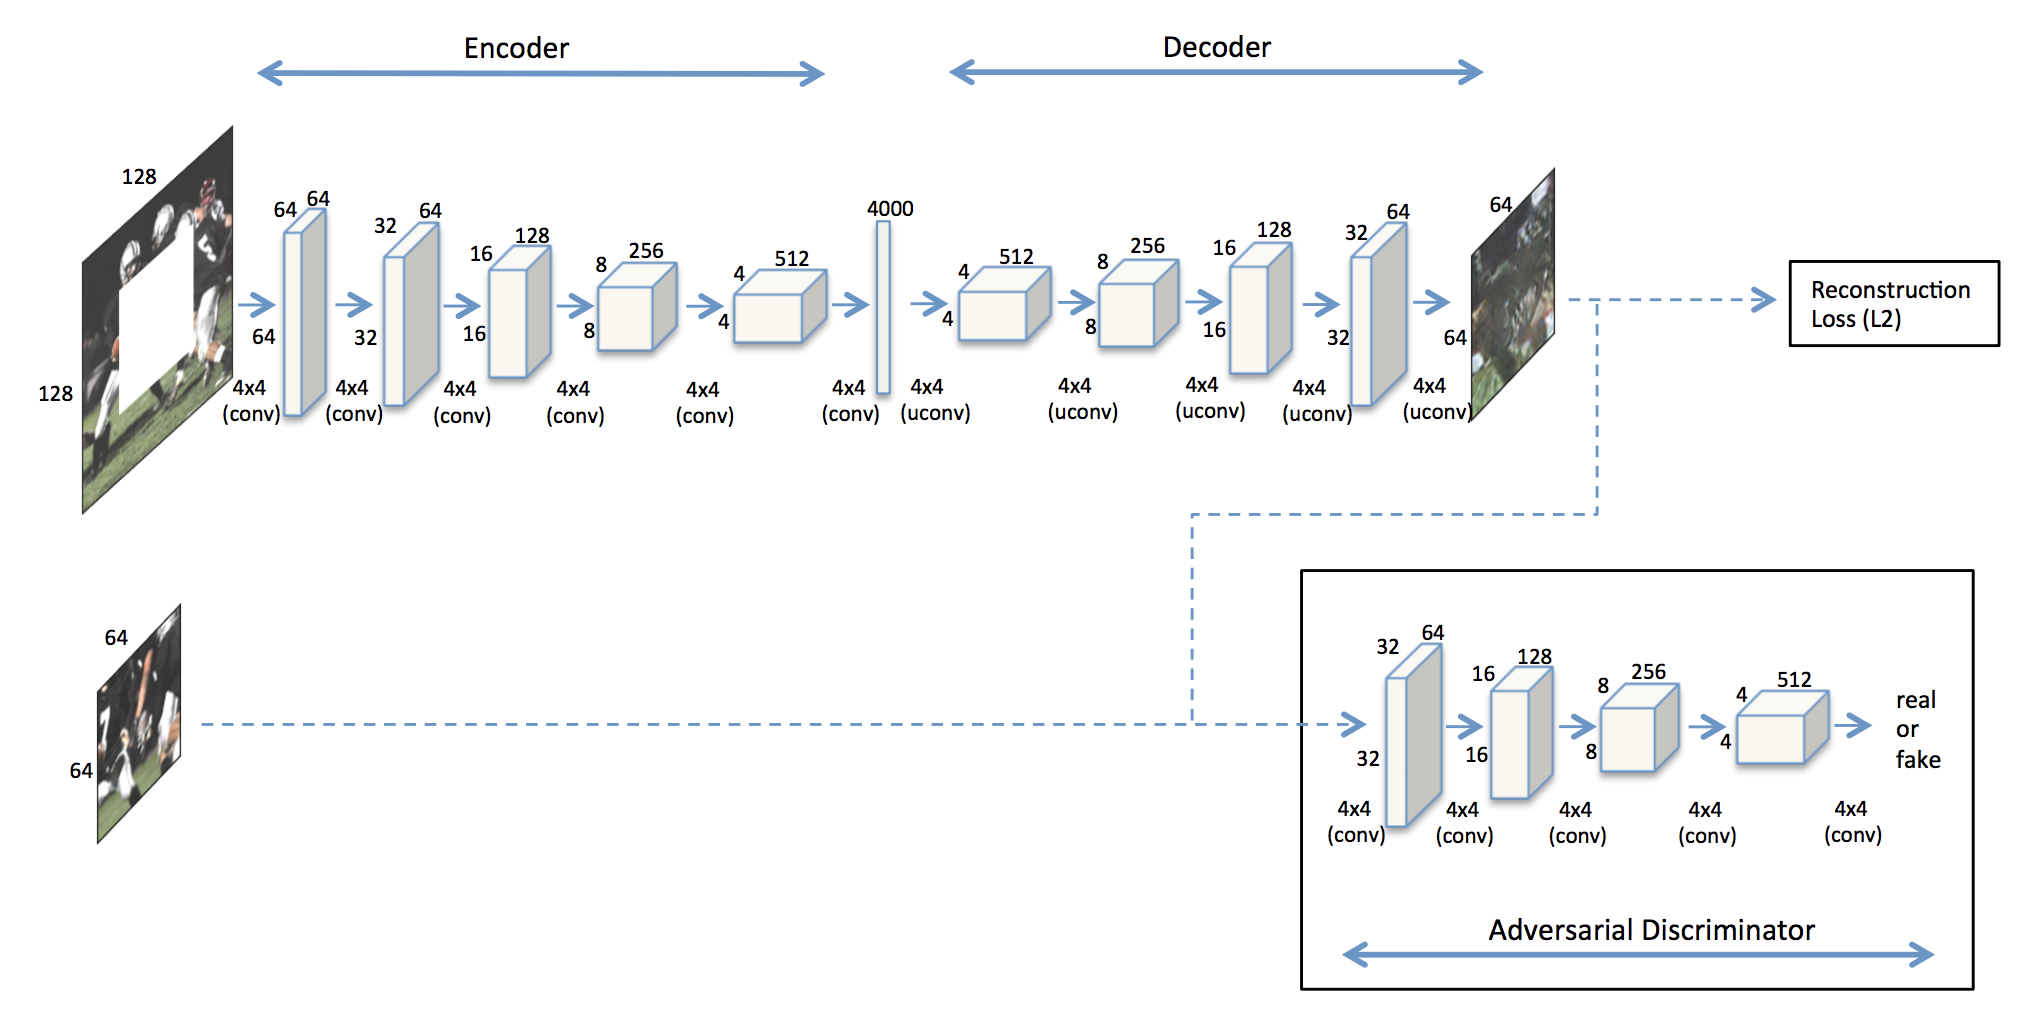
\includegraphics[width=1\linewidth,height=\textheight,keepaspectratio]{images/ssl/slide_21_1_img.png}
    \end{figure}

    \framebreak

    \begin{figure}
        \flushleft
        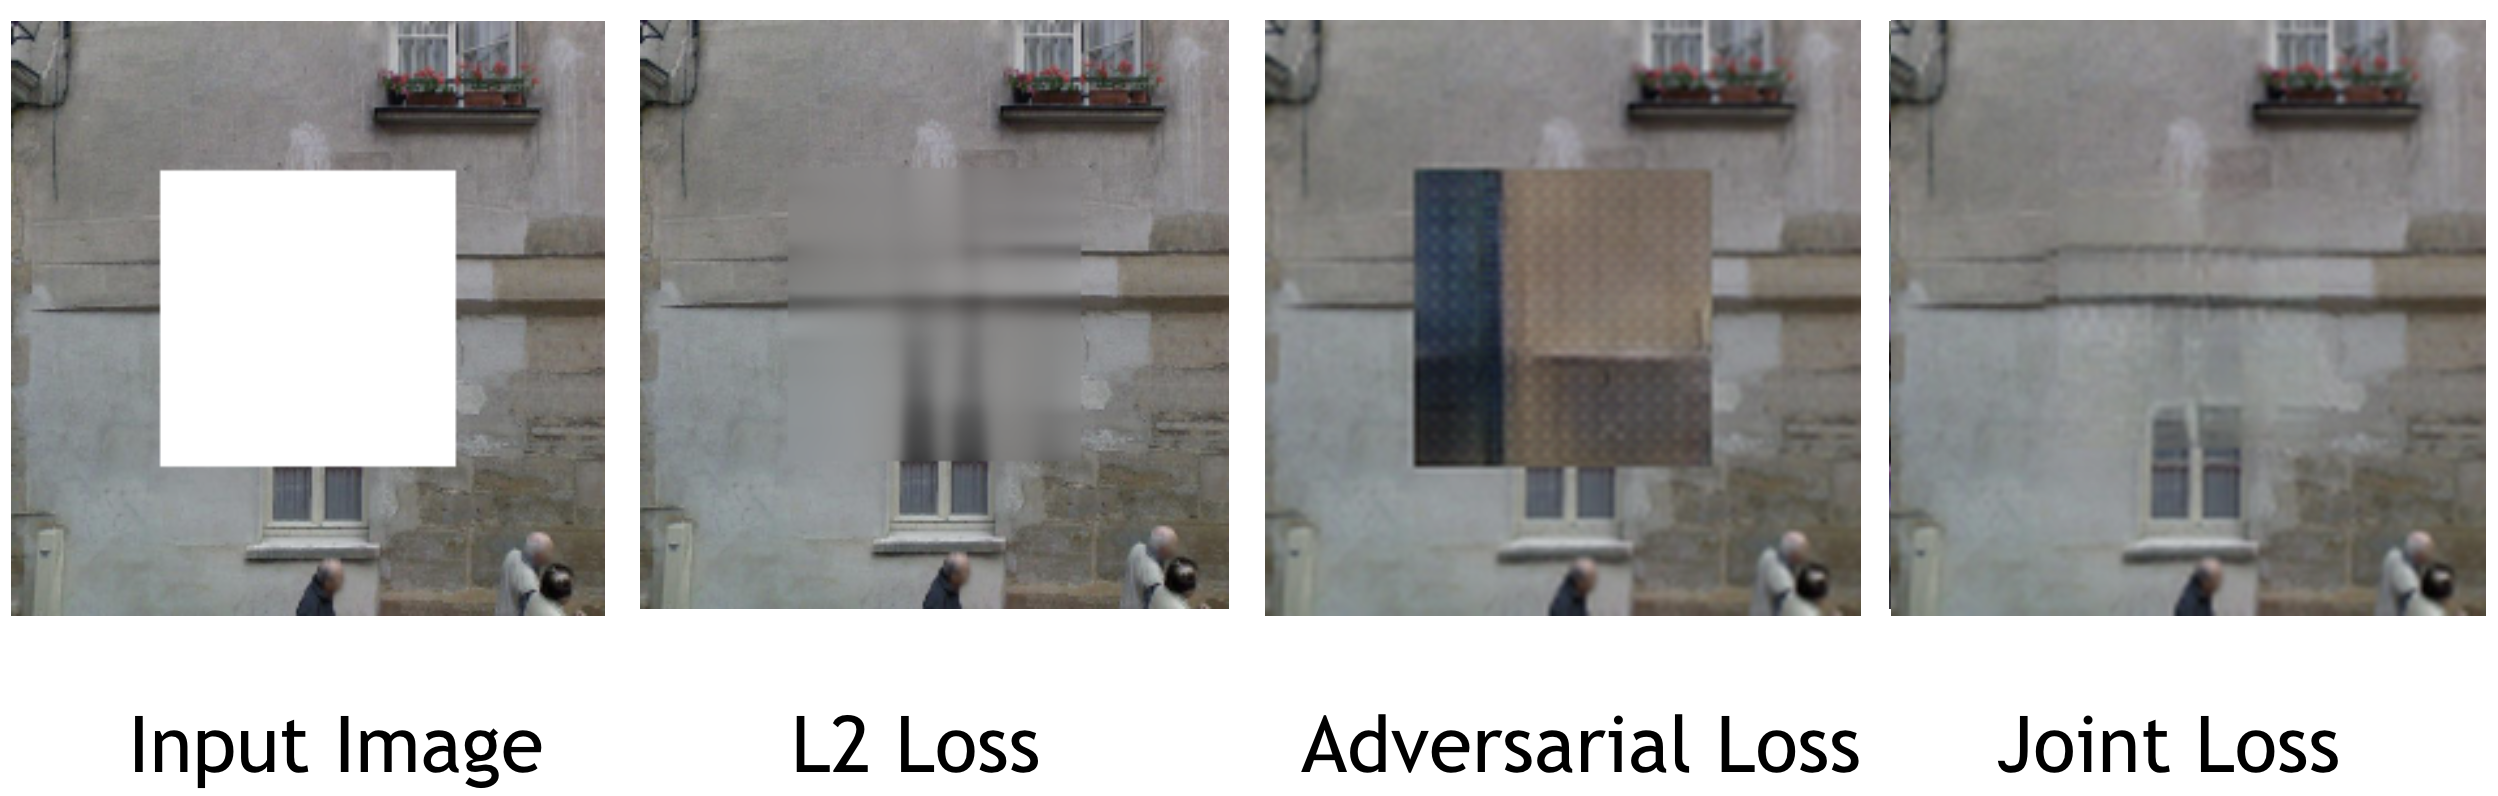
\includegraphics[width=1\linewidth,height=\textheight,keepaspectratio]{images/ssl/slide_22_1_img.png}
    \end{figure}

    \framebreak

    \begin{figure}
        \flushleft
        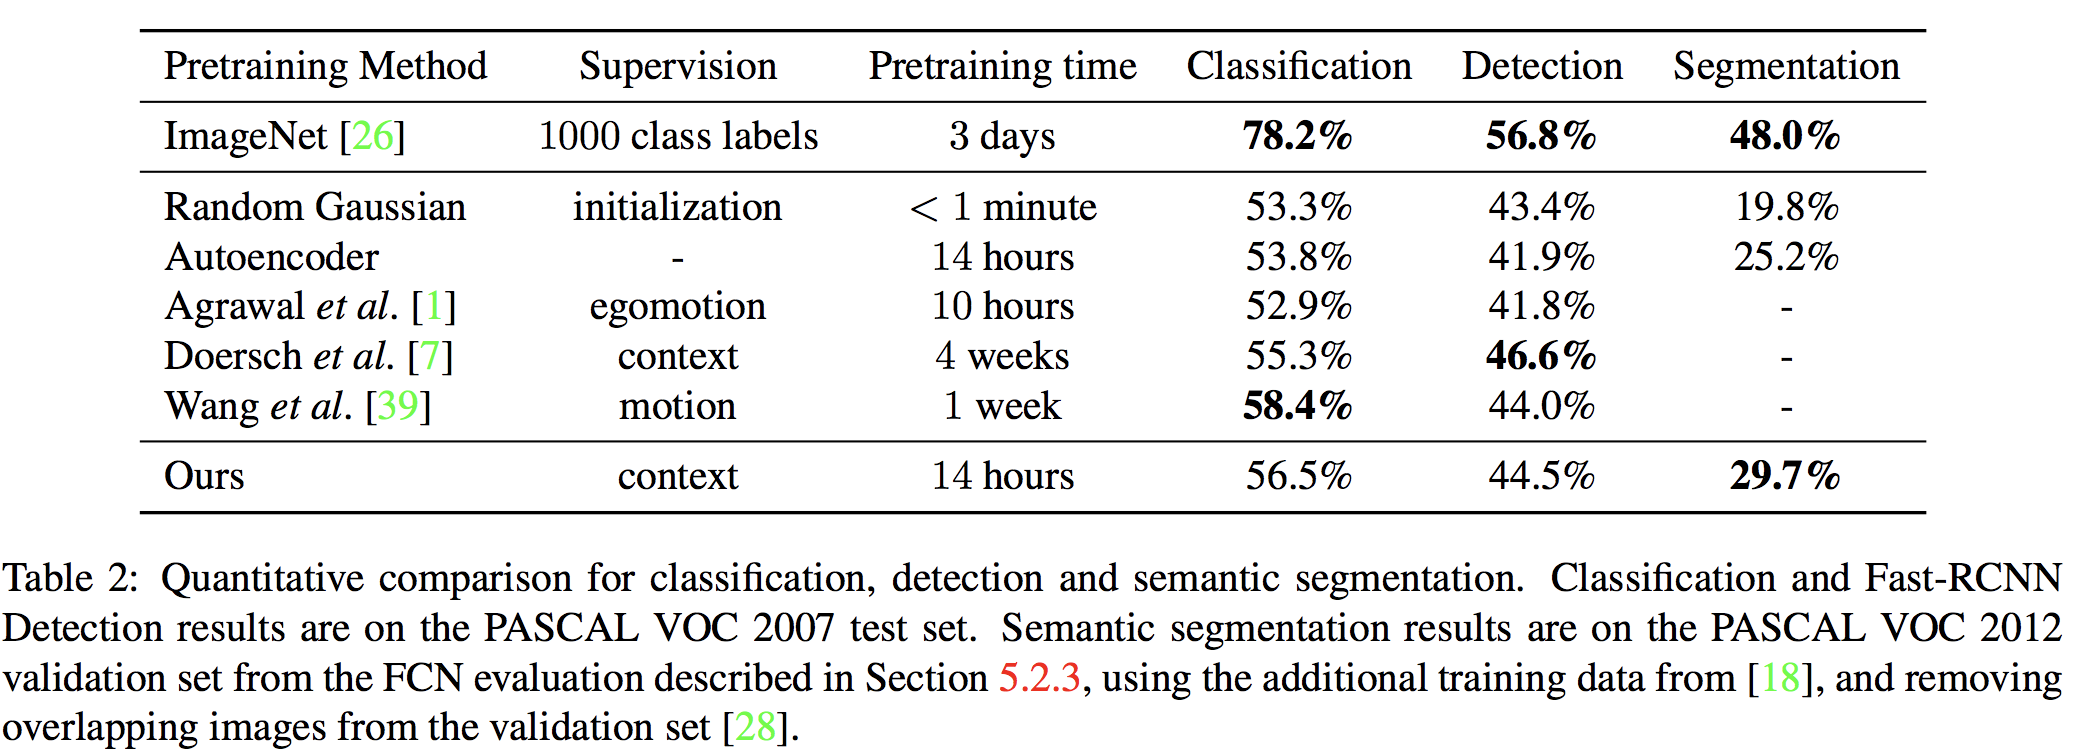
\includegraphics[width=1\linewidth,height=\textheight,keepaspectratio]{images/ssl/slide_23_1_img.png}
    \end{figure}

    \framebreak

    \vspace{0.5em}
    \textbf{Why does this work?}
    \begin{itemize}
        \setlength{\itemsep}{-0.25em}
        \item The network must understand the global and local context of the image to generate plausible content.
        \item This forces the model to learn semantic features and relationships within the image.
        \item The learned representations can be transferred to downstream tasks such as classification, detection, or segmentation.
    \end{itemize}

    \vspace{0.5em}
    \textbf{Applications:}
    \begin{itemize}
        \setlength{\itemsep}{-0.25em}
        \item Image inpainting
        \item Representation learning for transfer to other vision tasks
        \item Anomaly detection (by comparing predicted and actual content)
    \end{itemize}

    \vspace{0.5em}
    \textbf{Reference:}
    \begin{itemize}
        \item Pathak et al., "Context Encoders: Feature Learning by Inpainting," CVPR 2016.
    \end{itemize}
\end{frame}